\documentclass{article} 
%Grafiken einfügen
\usepackage{graphicx}
\usepackage{listings}

\setlength\parindent{0pt}

\begin{document} 
Dokumentation des {\LaTeX} Style für Berliner Debatte Initial.

\section{Anlegen eines neuen Hefts}

\subsection{Installation von \LaTeX}

\LaTeX ist ein Programm und eine Art der Dokumentauszeichnung. \LaTeX ermöglicht, wissenschaftliche Arbeiten zu verfassen ebenso wie Briefe, Präsentationen und auch Zeitschriften, wie die Berliner Debatte Initial. Die Idee dahinter ist eine Fokussierung auf die Inhalte zu ermöglichen und das Setzen des Textes beinahe vollständig zu automatisieren.

\LaTeX verwendet Befehle zum setzen des Textes. Jeder Befehl beginnt mit einen \textbackslash gefolgt von einem Wort, z.B. 

\begin{lstlisting}
    \chapter
\end{lstlisting}

für ein neues Kapitel. 

Formatierungen für die Inhalte werden von den Inhalten getrennt abgelegt und durch die entsprechenden Befehle auf die Inhalte angewendet, z.B. 

\begin{lstlisting}
    \newfontfamily{\chapterfont}{WarnockPro-Regular.otf}
    \renewcommand\huge{\@setfontsize\huge{20}{20}}
    \addtokomafont{chapter}{\chapterfont\huge}
\end{lstlisting}

um jede Kapitelüberschrift im gesamten Dokument mit der Schriftart Warnock-Pro Regular in Schriftgröße 20pt und einzeiligem Abstand zu setzen. 


\section{\LaTeX auf deinem Computer installieren}

Wichtig ist eine sogenannte \LaTeX Distribution herunterzuladen. Unter Windows empfiehlt sich Miktex\footnote{https://miktex.org/download/ctan/systems/win32/miktex/setup/windows-x64/basic-miktex-22.10-x64.exe}, unter MacOS empfiehlt sich MacTex\footnote{https://www.tug.org/mactex/mactex-download.html}

Das installieren von \LaTeX funktioniert genauso wie bei jedem anderen Programm, Pakete herunterladen und anklicken und dann warten bis die Installation fertig ist.

\subsection{\LaTeX Editor}

Darüber hinaus ist es sinnvoll einen Editor\footnote{https://www.texstudio.org/ Download für Windows oder Mac} zu installieren, mit dem du \LaTeX Dateien bearbeiten und kompilieren\footnote{Aus dem Textdokument das Heft erzeugen, ähnlich dem Übersetzen eines Textes von einer Sprache in eine andere Sprache} kannst. Den Editor musst du herunterladen und auf deinem Computer installieren.

\begin{figure}
    \centering
    \caption{Grundeinstellungen für ein neues Heft festlegen}
    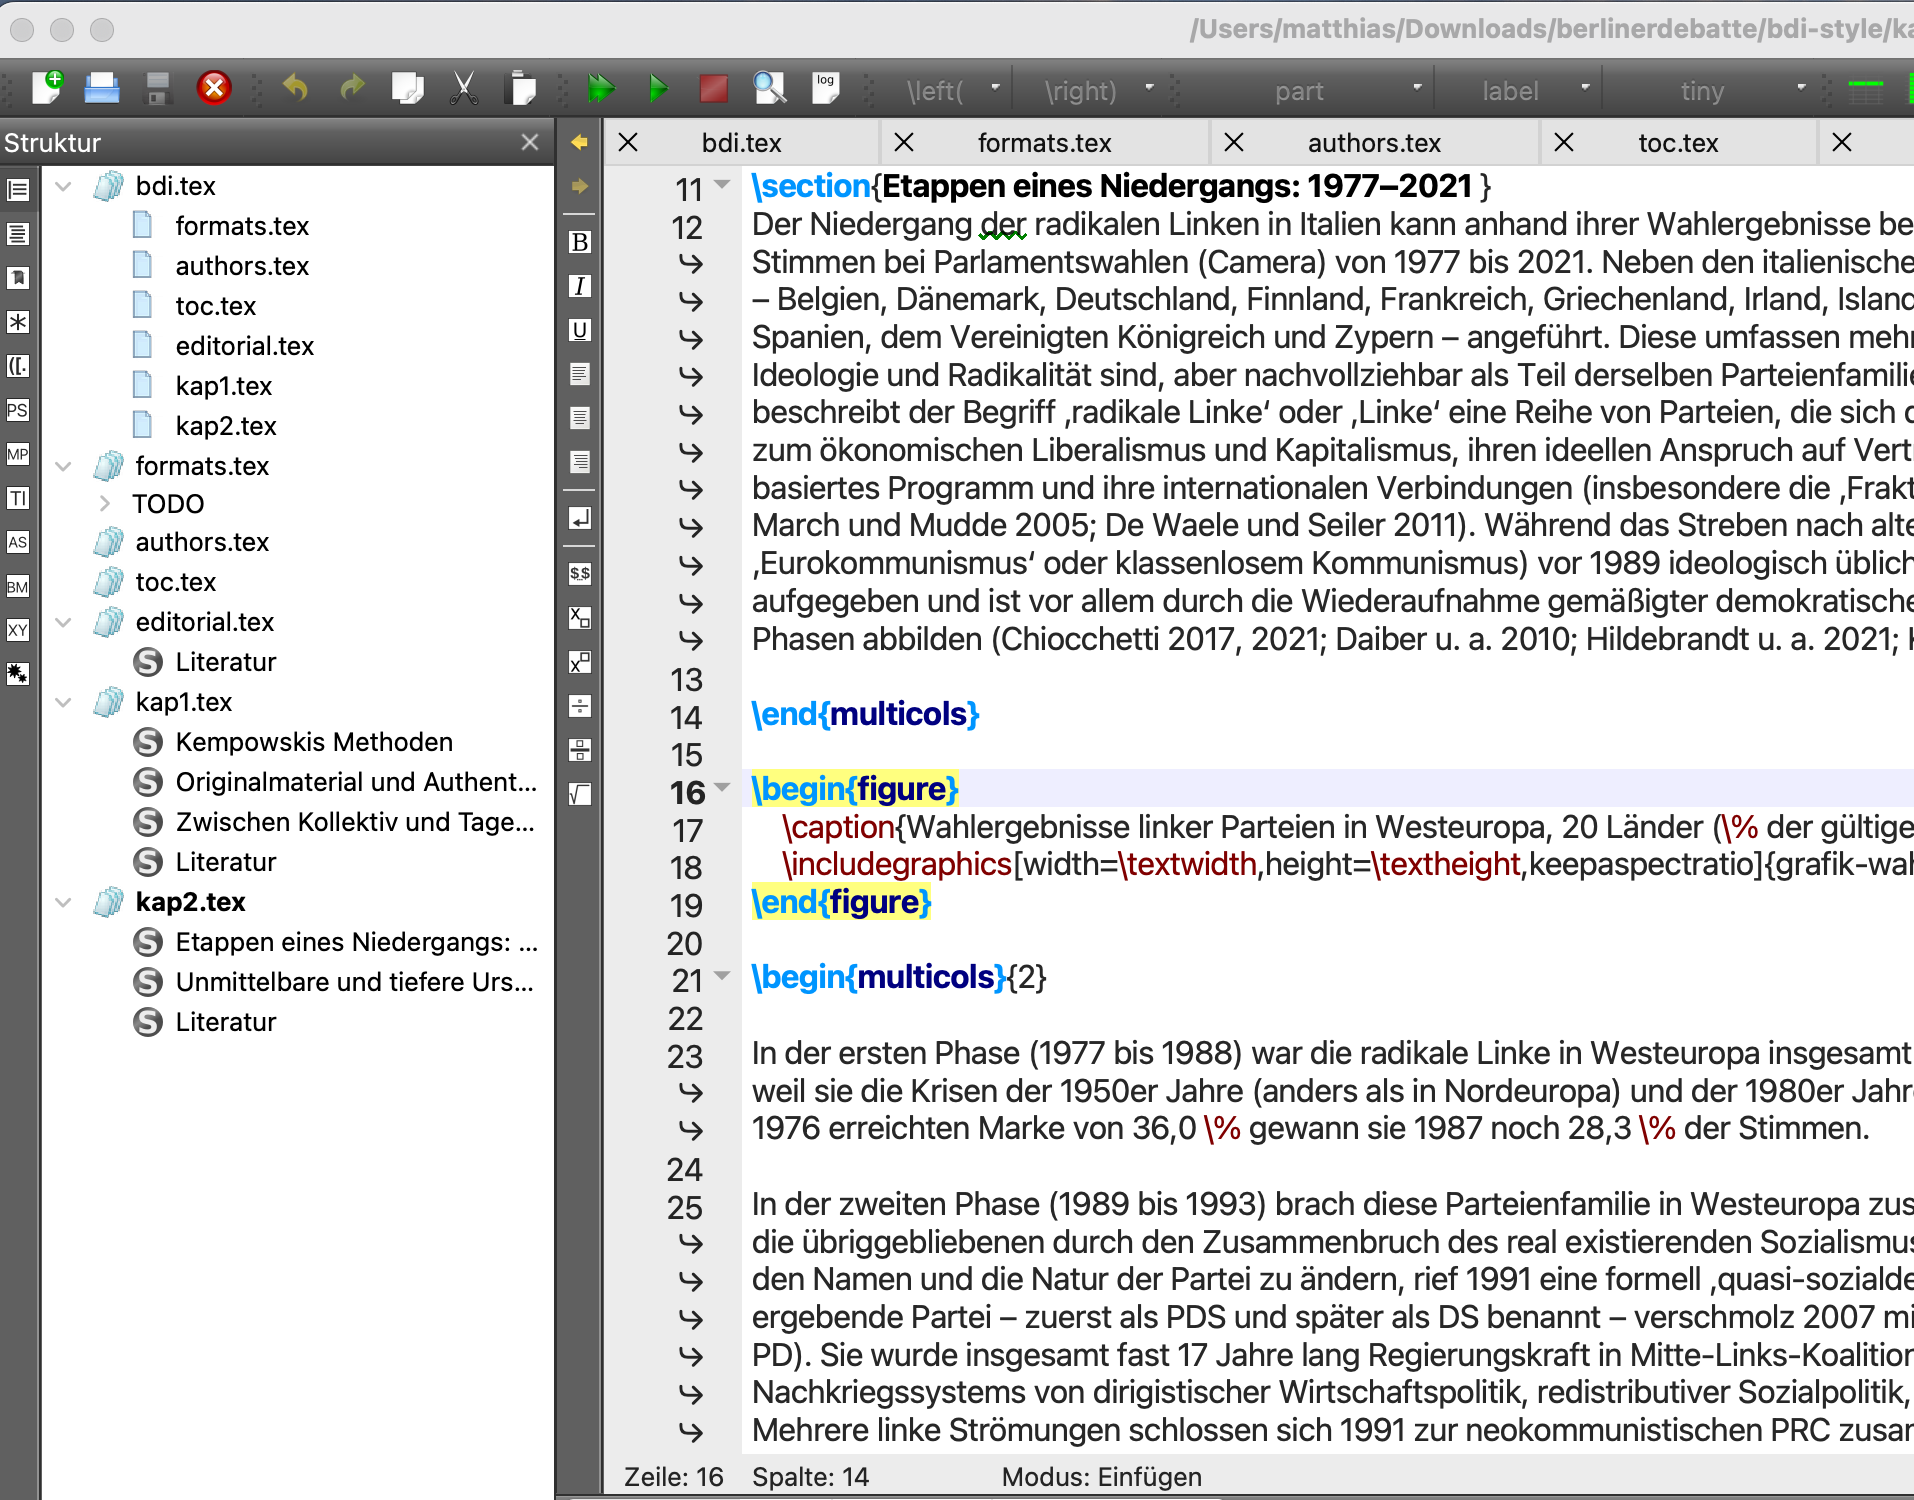
\includegraphics[scale=0.3]{texstudio.png}
\end{figure}

Da \LaTeX Dateien reine Textdateien sind hilft ein Editor dabei den Überblick zu behalten. So werden z.B. die Befehle farblich dargestellt und das Bauen der PDF Datei kann auch aus dem Editor heraus erfolgen. Ausserdem sieht man auf der linken Seite im Editor alle Dateien, die zum Projekt gehören.

\section{Vorlagen herunterladen}

Alle Vorlagen sind in einem öffentlich zugänglichen Speicher abgelegt. Um ein neues Heft zu erstellen gehe bitte auf github.com und lade dir das dazugehörige Paket herunter. Entpacke die Datei und starte den \LaTeX Editor. Öffne die Dateien, wie du es von Word oder Excel kennst. 

\section{Struktur der Vorlage}

Wenn du die Vorlage entpackt hast sind zwei neue Ordner entstanden. 

\begin{enumerate}
    \item bdi-Style
    \item cover
\end{enumerate}
   
Im Ordner "bdi-style" befinden sie alle Dateien für das Setzen des Heft Inhalts.

Im Ordner "cover" findest du alle Dateien, die notwendig sind um das Cover eines Hefts zu erstellen.

\subsection{Ordner bdi-style}

Das Herzstück eines Hefts sind die Dateien bdi.tex und formats.tex. 

\subsubsection*{formats.tex}

Diese Datei bitte {\bf nicht} bearbeiten!

\subsubsection*{bdi.tex}
In dieser Datei bitte in Zeile 9 ff. den Bereich Konfiguration anpassen und in die geschweifte Klammer die Werte für ein neues Heft eintragen. 

\begin{figure}
    \centering
    \caption{Grundeinstellungen für ein neues Heft festlegen}
    
\includegraphics[scale=0.8]{heftkonfiguration-festlegen.png}
\end{figure}

\begin{enumerate}
    \item Zeile 10: Jahrgang
    \item Zeile 11: Jahr
    \item Zeile 12: Ausgabe (Heftnummer)
\end{enumerate}

Aus den hier eingetragenen Werten ergibt sich automatisch die Ausgabe auf dem Buchrücken und in den Kopfzeilen der einzelnen Seiten. 

Weiter unten in der gleichen Datei werden die eigentlichen Inhalte des Hefts eingebunden.

\begin{figure}
    \centering
    \caption{Einbinden der Inhalte des Hefts}
    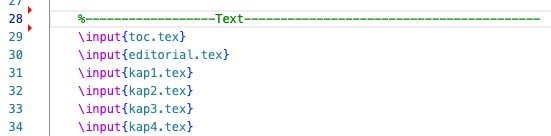
\includegraphics[scale=0.8]{Inhaltseinbindung.png}
\end{figure}

\begin{enumerate}
    \item toc.tex: Daraus wird das Inhaltsverzeichnis automatisch generiert
    \item kap1-x.tex: darin befinden sich die einzelnen Artikel des Hefts
\end{enumerate}

\section{Inhalte einfügen}

Um einen Artikel oder eine Rezension zu einem Heft hinzuzufügen sind folgende Schritte notwendig.

\begin{enumerate}
    \item Vorlage Artikel.tex oder Rezension.tex duplizieren und umbenennen
    \item Einbinden in der Datei bdi.tex
    \item Einfügen der Inhalte in die neu erstellte Datei
\end{enumerate}

\subsection{Erstellen eines Artikels}

Kopiere die Vorlage Artikel.tex und benenne sie entsprechend um in "Name-des-Artikels.tex. Anschließend gehe in die Datei bdi.tex und binde die Vorlage wie weiter oben beschrieben ein.

In der Vorlage findest du alle notwendigen Informationen um einen normalen Text ohne Bilder und Tabellen richtig zu setzen. 

\subsection{Erstellen eines Rezension}

Kopiere die Vorlage Rezensionen.tex und benenne sie entsprechend um in z.B. rezensionen.tex. Anschließend gehe in die Datei bdi.tex und binde die Vorlage wie weiter oben beschrieben ein.

In der Vorlage findest du alle notwendigen Informationen um einen normalen Text ohne Bilder und Tabellen richtig zu setzen. 

\subsection{Überschriften Editorial}

\begin{lstlisting}
    \bdieditorial{Johanna Wischner, Thomas Müller}
\end{lstlisting}

\textbf{Resultat} ist die gesetzte Überschrift eines Editorials.

\begin{center}
    
\includegraphics[scale=0.5]{editorial-headline.png}
\end{center}

\subsection{Überschriften Artikel}

\begin{lstlisting}
    \bdichapter{<AUTOREN>}{<>TITEL}{<FORMATIERTER TITEL>}{<UNTERTITEL>}
\end{lstlisting}

\textbf{Resultat} ist die gesetzte Überschrift eines Artikels.

\begin{center}
    
\includegraphics[scale=0.5]{rezensionen-headline.png}
\end{center}

\subsection{Überschriften Rezensionen}

\begin{lstlisting}
    \bdirezension{Sonia Combe}{Loyal um jeden Preis.\smallskip „Linientreue Dissidenten“ im Sozialismus}{Ulrich Busch}
\end{lstlisting}

\textbf{Resultat} ist die gesetzte Überschrift einer Rezension.

\begin{center}
    
\includegraphics[scale=0.5]{bdichapter.png}
\end{center}

\subsection{Absätze ohne Einrückung}

\begin{lstlisting}
    \noindent Jemand musste Josef K. 

    Jemand musste Josef K. 
\end{lstlisting}

\textbf{Resultat} ist das der Absatz nicht eingerückt wird. Der darauf folgende Absatz wird normal eingerückt.

\begin{center}
    
\includegraphics[scale=0.4]{noindent.png}
\end{center}

\subsection{Fettdruck und Kursivschrift}

\begin{lstlisting}
    Ein \textbf {großer Teil} des \textit{unveröffentlichten 
    Materials}, das in 
\end{lstlisting}

\textbf{Resultat} ist das die Worte in der Klammer nach dem Befehl Fett oder Kursiv ausgegeben werden.

\begin{center}
    
\includegraphics[scale=0.4]{fett-kursiv.png}
\end{center}

\subsection{Endnoten}

\begin{lstlisting}
    Vom Archiv zur Druckfassung\endnote{Übersetzte und 
    überarbeitete Fassung von „Walter Kempowski’s Das Echolot. 
    Abgesang ’45. From Archive to Print“, erschienen in: German 
    Life and Letters 66 (2013), Heft 4, S. 416-431 (German Life 
    and Letters © John Wiley \& Sons Ltd.). Mit freundlicher 
    Genehmigung des Verlags.}
\end{lstlisting}

\textbf{Resultat} ist das an der Stelle wo die Endnote im Text eingefügt wurde ein Nummer erscheint und am Ende des Textes die Endnote ausgegeben wird.

\begin{center}
    
\includegraphics[scale=0.4]{nummerierung-endnote.png}
\end{center}

\begin{center}
    
\includegraphics[scale=0.4]{endnote.png}
\end{center}

\subsection{Bibliografie}

\begin{lstlisting}
    begin{bibdescription}
        \item Franz Kafka, Der Prozess
        \item Eintrag 2
        \item Eintrag 3 
        \item etc. pp.
    \end{bibdescription}
\end{lstlisting}

\textbf{Resultat} ist eine fortlaufende und unnummerierte Liste der Literaturangaben.

\begin{center}
    
\includegraphics[scale=0.4]{literaturverzeichnis.png}
\end{center}

\subsection{Bilder}

\begin{lstlisting}
    \begin{figure*}
        \centering
        \caption{Stilisierte politische Einstellungen von 
        Gruppen mit hohem Bildungsniveau 
        (nach Kitschelt, Rehm 2022)}
        \includegraphics[scale=0.8]{brie-2.eps} 
    \end{figure*}
\end{lstlisting}

\textbf{Resultat} ein eingebundenes Bild mit einem Titel. Im Befehl oben siehst du, dass du die Bildgröße anpassen kannst durch die Angabe scale, der Wert 0.8 bedeutet: skaliere das Bild auf 80\% Größe.

Die Formate der Bilder sollten .png, .jpg oder .eps sein. Die Beste Qualität für den Ausdruck bietet das .eps Format, da es sich hierbei um eine skalierbare Vektorgrafik handelt.

\begin{center}
    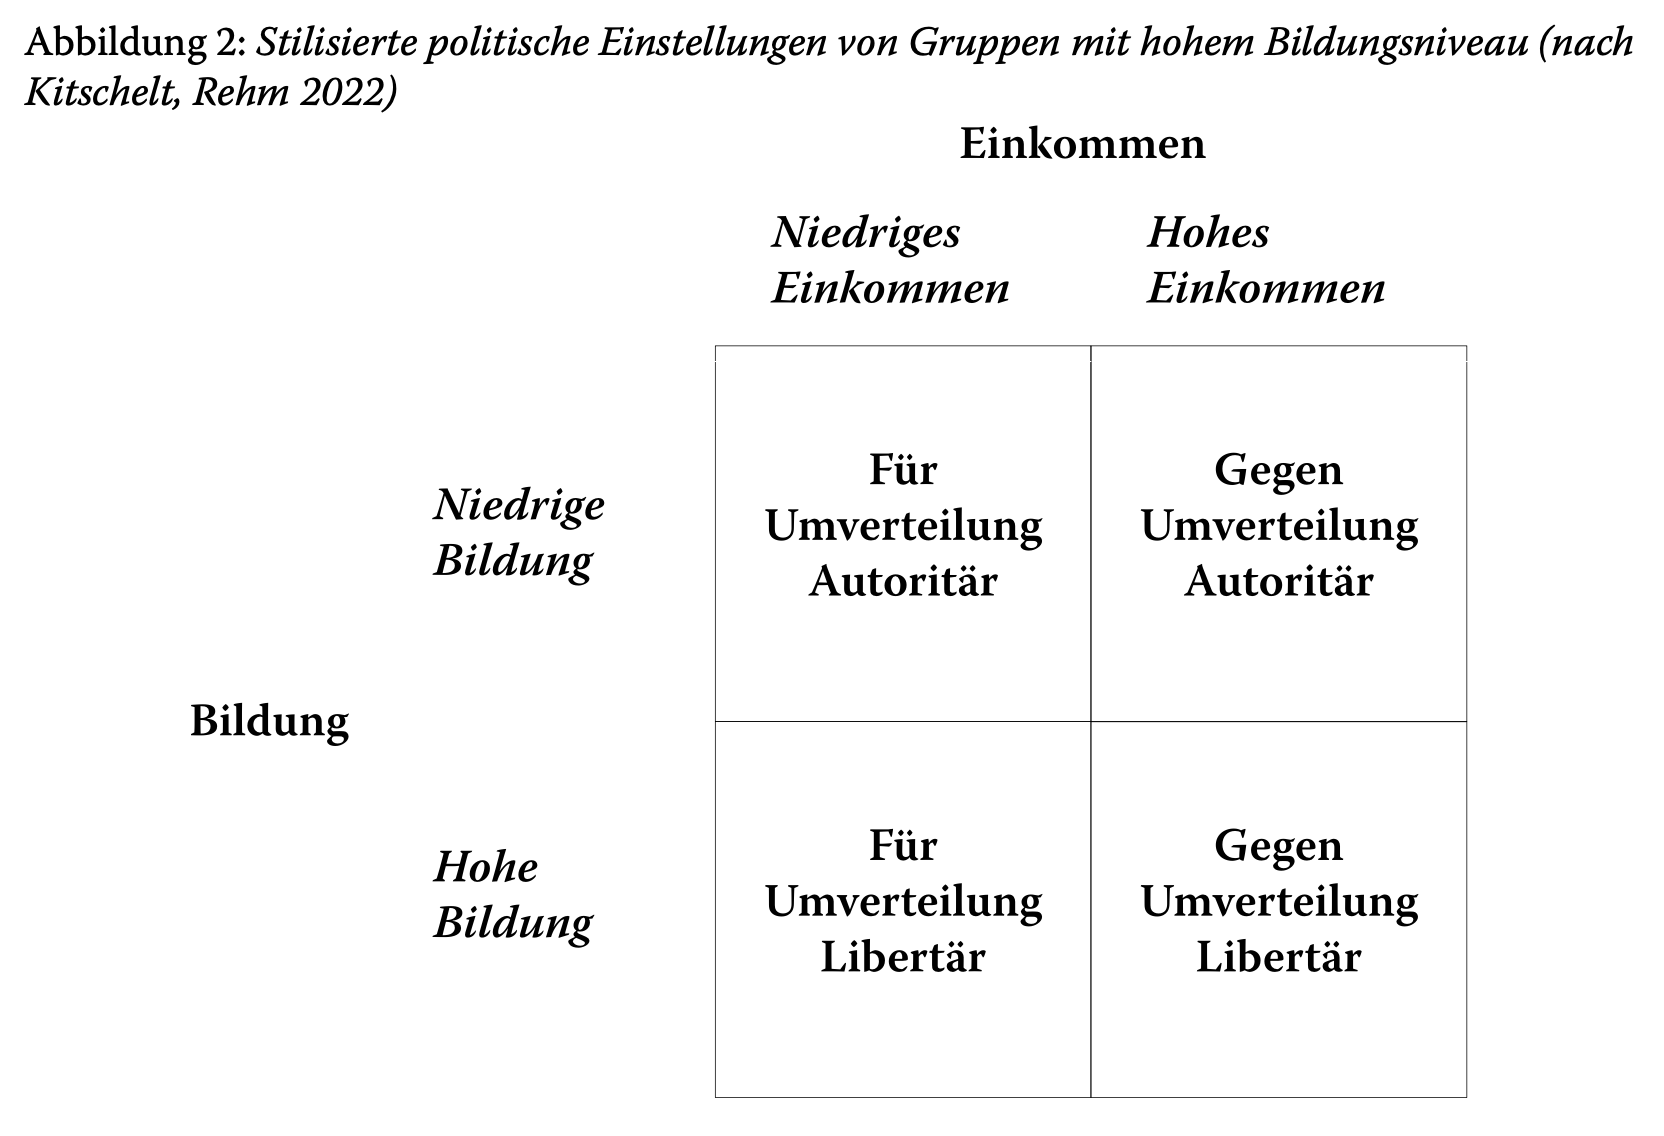
\includegraphics[scale=0.4]{bilder.png}
\end{center}

\subsection{Tabellen}

Tabellen sind ein etwas komplexeres Thema. Tabellen sind in \LaTeX grundsätzlich so aufgebaut:

\begin{lstlisting}
    \begin{tabular*}
        \begin{tabular}{l|c|r}
            1 & 2 & 3 \\\hline
            4 & 5 & 6 \\
            7 & 8 & 9 \\
        \end{tabular}
    \end{tabular*}
\end{lstlisting}

\begin{enumerate}
    \item {tabular*}: startet eine Umgebung, die sich an der passenden Stelle in den Text einklinkt und aus zwei Spalten eine macht.
    \item {tabular}{l|c|r}: startet die Tabelle und definiert die Anzahl der Spalten. Die Werte l, c, r stehen für die Ausrichtung des Texts innerhalb der Spalte.
    \item 1 \& 2 \& 3 \textbackslash\textbackslash: die Zahlen sind der Inhalt der Tabelle, das \& ist der Spaltentrenner und \textbackslash\textbackslash sind der Umbruch in die näcshte Tabellenzeile.
    \item \textbackslash hline am ende der ersten Zeile setzt eine horizontale Linie unter die erste Zeile.
\end{enumerate}

\textbf{Resultat} ist eine Tabelle mit 3 Spalten und 3 Zeilen, die erste Spalte hat eine Linie unten.  

\vspace{1cm}
    \begin{tabular}{l|c|r}
        1 & 2 & 3 \\\hline
        4 & 5 & 6 \\
        7 & 8 & 9 \\
    \end{tabular}
\vspace{1cm}

Komplexere Tabellen sollten idealerweise nicht manuell eingegeben werden, da die Wahrscheinlichkeit einen Fehler zu machen recht hoch ist. Es existiert ein Onlinetool "Table Maker", dort können Tabellen aus Word oder Excel einfach reinkopiert werden und eine \LaTeX Übersetzung erstellt werden, die dann von dort einfach ins \LaTeX Dokument kopiert wird. (URL: https://www.latex-tables.com/v3/index.html) 

\begin{center}
    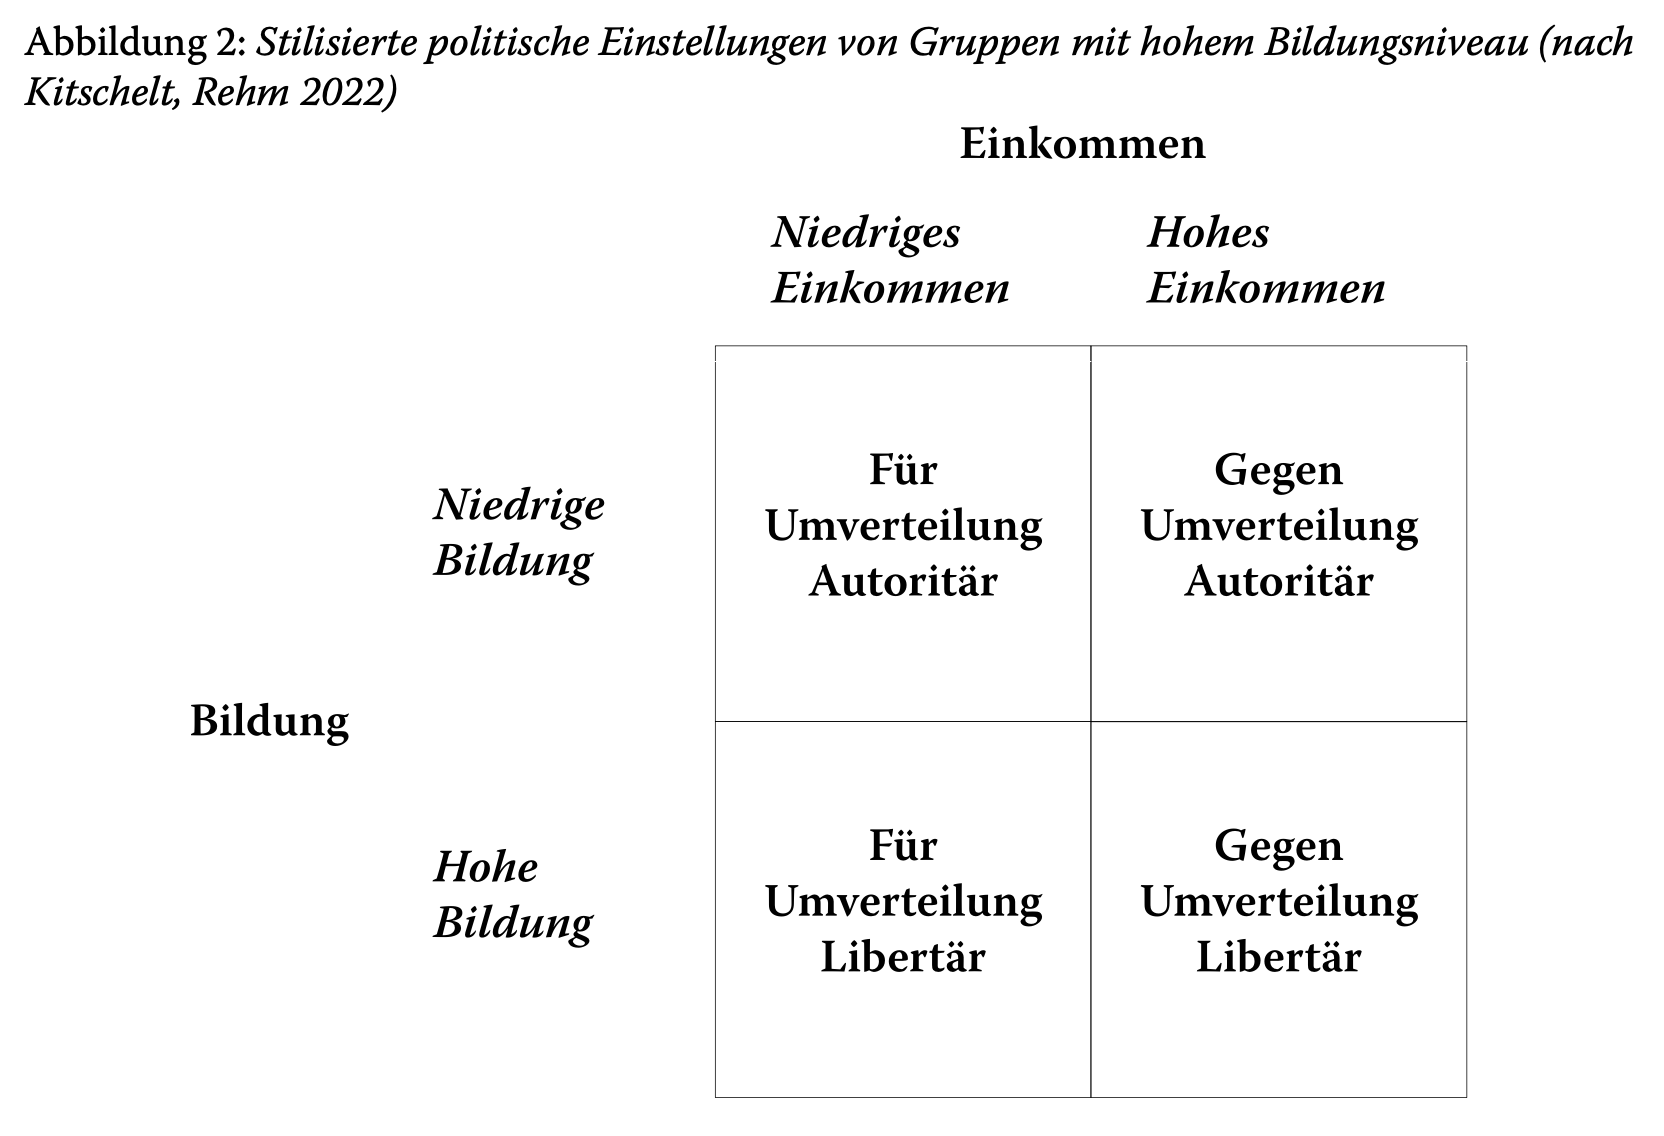
\includegraphics[scale=0.4]{bilder.png}
\end{center}


Hier findest du folgende Dateien zum Bearbeiten vor. 

\begin{enumerate}
    \item formats.tex
    \item bdi.tex
    \item hyphenation.tex
    \item toc.tex
\end{enumerate}


\end{document}

